\documentclass[10pt,a4paper]{article}
%]{report}

\usepackage[a4paper, top=2cm, bottom=2.5cm, left=3cm, right=3cm]{geometry}
%\usepackage[
%    vmarginratio=2:2.5, %Verh�ltnis der oben/unten Seitenr�nder zur automatischen Berechnung
%    paper=a4paper,
%    lmargin=3cm, % mittlerer Rand
%    rmargin=3cm, % �u�erer Rand
%    marginparwidth=2.3cm, % Breite des Marginpars
%    includehead, % Kopfzeile in Berechnung einbeziehen
%    includemp % Marginpar in die Berechnung mit einbeziehen
%]{geometry}
%\setlength\marginparwidth{2.3cm} %Die wird sp�ter zum Rechnen gebraucht, wird aber durch die Angabe im geometry package nicht automatisch richtig gesetzt.


%============================================================
% Pakete
%============================================================

\usepackage[english, ngerman]{babel}    % mehrsprachiger Textsatz
% babel: letzte Sprache in Optionen zeigt die Sprache des Dokumentes
% und kann durch den Befehl \selectlanguage{} geaendert werden
% Passen Sie die Optionen des babel-Paketes nach Bedarf an!
\usepackage[utf8]{inputenc}       % Eingabekodierung Parameter latin1 darf ge�ndert werden
\usepackage[T1]{fontenc}                % Schriftenkodierung
\usepackage{graphicx}                       % zum Einbinden von Grafiken
\usepackage{lmodern}                        % Ersatz fuer Computer Modern-Schriften
                                                                % zum besseren Aussehen am Bildschirm
\usepackage{epstopdf}		% Grafiken einbinden
\usepackage{caption}		%Grafiken beschriften
%\usepackage{verbatimfiles}	% Ganze Dateien als Verbatim einbinden
% \usepackage{programs}	% Ganze Dateien als Verbatim einbinden
\usepackage{verbatim}		% Mehrzeilige Kommentare
\usepackage{multicol}		% Mehrere Spalten
\usepackage{hyphsubst}		% Silbentrennung
\usepackage{xcolor,soul}
\usepackage{float}				%Sachen an der richtigen Stelle ausgeben
\restylefloat{figure}				%Abbildungen an der richtigen Stelle ausgeben
\restylefloat{table}				%Tabellen an der richtigen Stelle ausgeben
\usepackage{array}				%f�r Tabellen
\newcolumntype{C}{>{$}c<{$}} 	%Tabellenspalten C mit mathematischem Inhalt
\usepackage{subfigure}
\usepackage{ulem}				%doppelt unterstreichen
\usepackage{siunitx}
\usepackage{hyperref}
\usepackage{booktabs}


\usepackage{etex} %needs to be used to avoid 'no room error in pgfplots'
\usepackage{pgfplots}
\usepackage{tikz}
\usepackage{tikz-3dplot}
%\usepackage{tikzscale}
\usepgfplotslibrary{polar}
\usetikzlibrary[pgfplots.colormaps]
\pgfplotsset{compat=newest}
\pgfplotsset{plot coordinates/math parser=false}
\newlength\figureheight
\newlength\figurewidth
%\pgfplotsset{y tick label style={/pgf/number format/fixed}}
%\pgfplotsset{yticklabel style={text width=2.2em,align=right}}%,fixed zerofill, precision=1}}
%\pgfplotsset{every x tick/.append style={line width=1pt}}
%\pgfplotsset{every y tick/.append style={line width=1pt}}
%\pgfplotsset{every axis plot/.append style={line width=1.0pt}}
%\pgfplotscreateplotcyclelist{mycolorlist}{blue,red,green,brown,teal,orange,violet,cyan,green!70!black,magenta,gray}

\usepackage{tikzscale}
\usetikzlibrary{external}
\usetikzlibrary{fadings}
\usetikzlibrary{arrows}
\usetikzlibrary{calc}
\usetikzlibrary{plotmarks}
\usepgfplotslibrary{external}
\tikzset{external/force remake=false}
\tikzset{external/system call={pdflatex \tikzexternalcheckshellescape -halt-on-error -interaction=batchmode -jobname "\image" "\texsource"}}

\tikzexternalize

% define colors for source code list
\definecolor{colKeys}{rgb}{0,0,1}
\definecolor{colIdentifier}{rgb}{0,0,0}
\definecolor{colComments}{rgb}{0,1,0.3}
%\definecolor{colString}{rgb}{0,0.5,0}
\definecolor{dkgreen}{rgb}{0,0.6,0}
\definecolor{gray}{rgb}{0.5,0.5,0.5}
\definecolor{colString}{rgb}{0.63,0.13,0.94}

% Code-Listings print source code
\usepackage{listings}
\lstset{language=Python,		% choose the language of the code
	inputencoding=latin1,
	keywords={break,case,catch,continue,else,elseif,end,for,function,
	 global,if,otherwise,persistent,return,switch,try,while,ones,zeros},
   	float=hbp,
%  	 basicstyle=\ttfamily\small,				% the size of the fonts that are used for the code
   	identifierstyle=\color{colIdentifier},
   	keywordstyle=\color{blue},
   	commentstyle=\color{dkgreen},
  	stringstyle=\color{colString},
   	columns=flexible,
  	tabsize=2,								% sets default tabsize to 2 spaces
   	%frame=none; %single,
  	 numbers=left,						% where to put the line-numbers
  	 showspaces=false,                               % show spaces adding particular underscores
  	 numberstyle=\ttfamily\small\color{gray},
% numberstyle=\footnotesize,                      % the size of the fonts that are used for the line-numbers
  	 stepnumber=1,                                           % the step between two line-numbers. If it's 1 each line will be numbered
  	 numbersep=10pt,                                  % how far the line-numbers are from the code
  	 showspaces=false,
  	 showstringspaces=false,                         % underline spaces within strings
  	 breakautoindent=true,                        % sets if automatic breaks should only happen at whitespace
%       backgroundcolor=\color{white},          % choose the background color. You must add \usepackage{color}
%  	     showtabs=false,                                         % show tabs within strings adding particular underscores
%       frame=single,                                           % adds a frame around the code
%       captionpos=b,                                           % sets the caption-position to bottom
%        escapeinside={\%*}{*)                          % if you want to add a comment within your code
        breaklines=true}                                       % sets automatic line breaking

% Mathe-Pakete
\usepackage{amsfonts}
\usepackage{amsmath}
\usepackage{amsthm}		% Theorem-Umgebung, Beweise
\usepackage{amssymb}
\usepackage{cancel}
\usepackage{mathcomp}
\usepackage{nicefrac}

\usepackage{libertine}
\usepackage[libertine]{newtxmath}

%============================================================
% Titel, Autor, Datum
%============================================================
\title{Übung 3 \\Computational Physics III}
\author{Matthias Plock (552335) \and Paul Ledwon (561764)} %\\Otto Normalverbraucher (271828)}
\date{\today}

%============================================================
% Dokument
%============================================================
\begin{document}

% Titel erstellen
\maketitle
\tableofcontents

\pagenumbering{arabic}
\pagestyle{myheadings}                  % bzw. ist fancyhdr zu benutzten

\section{Aufgabe 1}

Auf der GPU wird die Addition von Arrays der Dimension $N=1024^2$ für verschiedene execution configurations, daher die Einteilung der Threads in zweidimensionale Blöcke und Grids untersucht. Der untersuchte Parameter ist die Laufzeit der Vektoraddition.
Die Dimension $N$ wird als Produkt von vier Faktoren dargestellt, wobei die Faktoren die
Aufteilung in Block- und Gridgröße bestimmen.
Tendenziell scheinen Verteilungen mit großen Griddimensionen und kleinen Blockdimensionen die kürzesten Laufzeiten zu haben.
Aus den 820 möglichen Kombinationen werden die 40 schnellsten execution configurations aufgelistet:

\begin{verbatim}
0.00016 seconds for 	 gridX: 2 	 gridY: 262144 	 threadX: 2 	 threadY: 1
0.00016 seconds for 	 gridX: 131072 	 gridY: 1 	 threadX: 2 	 threadY: 4
0.00016 seconds for 	 gridX: 1 	 gridY: 262144 	 threadX: 1 	 threadY: 4
0.00016 seconds for 	 gridX: 2 	 gridY: 65536 	 threadX: 8 	 threadY: 1
0.00016 seconds for 	 gridX: 262144 	 gridY: 1 	 threadX: 4 	 threadY: 1
0.000161 seconds for 	 gridX: 65536 	 gridY: 2 	 threadX: 8 	 threadY: 1
0.000161 seconds for 	 gridX: 65536 	 gridY: 4 	 threadX: 1 	 threadY: 4
0.000161 seconds for 	 gridX: 65536 	 gridY: 4 	 threadX: 4 	 threadY: 1
0.000161 seconds for 	 gridX: 131072 	 gridY: 4 	 threadX: 2 	 threadY: 1
0.000161 seconds for 	 gridX: 1 	 gridY: 524288 	 threadX: 2 	 threadY: 1
0.000161 seconds for 	 gridX: 1 	 gridY: 131072 	 threadX: 8 	 threadY: 1
0.000161 seconds for 	 gridX: 131072 	 gridY: 4 	 threadX: 1 	 threadY: 2
0.000161 seconds for 	 gridX: 524288 	 gridY: 1 	 threadX: 2 	 threadY: 1
0.000161 seconds for 	 gridX: 65536 	 gridY: 2 	 threadX: 4 	 threadY: 2
0.000161 seconds for 	 gridX: 1 	 gridY: 131072 	 threadX: 2 	 threadY: 4
0.000161 seconds for 	 gridX: 1 	 gridY: 131072 	 threadX: 1 	 threadY: 8
0.000161 seconds for 	 gridX: 131072 	 gridY: 2 	 threadX: 4 	 threadY: 1
0.000161 seconds for 	 gridX: 131072 	 gridY: 1 	 threadX: 8 	 threadY: 1
0.000161 seconds for 	 gridX: 65536 	 gridY: 8 	 threadX: 2 	 threadY: 1
0.000161 seconds for 	 gridX: 65536 	 gridY: 8 	 threadX: 1 	 threadY: 2
0.000161 seconds for 	 gridX: 1 	 gridY: 65536 	 threadX: 1 	 threadY: 16
0.000161 seconds for 	 gridX: 1 	 gridY: 65536 	 threadX: 2 	 threadY: 8
0.000161 seconds for 	 gridX: 1 	 gridY: 131072 	 threadX: 4 	 threadY: 2
0.000161 seconds for 	 gridX: 1 	 gridY: 65536 	 threadX: 8 	 threadY: 2
0.000161 seconds for 	 gridX: 262144 	 gridY: 1 	 threadX: 1 	 threadY: 4
0.000161 seconds for 	 gridX: 65536 	 gridY: 2 	 threadX: 1 	 threadY: 8
0.000161 seconds for 	 gridX: 524288 	 gridY: 1 	 threadX: 1 	 threadY: 2
0.000161 seconds for 	 gridX: 8 	 gridY: 65536 	 threadX: 2 	 threadY: 1
0.000161 seconds for 	 gridX: 8 	 gridY: 65536 	 threadX: 1 	 threadY: 2
0.000161 seconds for 	 gridX: 4 	 gridY: 131072 	 threadX: 2 	 threadY: 1
0.000161 seconds for 	 gridX: 4 	 gridY: 131072 	 threadX: 1 	 threadY: 2
0.000161 seconds for 	 gridX: 4 	 gridY: 65536 	 threadX: 4 	 threadY: 1
0.000161 seconds for 	 gridX: 262144 	 gridY: 2 	 threadX: 1 	 threadY: 2
0.000161 seconds for 	 gridX: 2 	 gridY: 262144 	 threadX: 1 	 threadY: 2
0.000161 seconds for 	 gridX: 2 	 gridY: 131072 	 threadX: 4 	 threadY: 1
0.000161 seconds for 	 gridX: 4 	 gridY: 65536 	 threadX: 1 	 threadY: 4
0.000161 seconds for 	 gridX: 2 	 gridY: 65536 	 threadX: 4 	 threadY: 2
0.000161 seconds for 	 gridX: 2 	 gridY: 65536 	 threadX: 2 	 threadY: 4
0.000161 seconds for 	 gridX: 65536 	 gridY: 1 	 threadX: 2 	 threadY: 8
0.000161 seconds for 	 gridX: 65536 	 gridY: 1 	 threadX: 16 	 threadY: 1
\end{verbatim}

Mit einer Laufzeit von $160\thinspace\mu$s ist die Konfiguration mit \num{2} $\cdot$ \num{262144} Blöcken und \num{2} $\cdot$ \num{1} Threads am schnellsten. Die langsameren Konfigurationen waren alle bei unter $700\thinspace\mu$s.
Die schnellsten \num{40} execution configurations haben gerade die Eigenschaft, dass eine Blockdimension groß gegenüber der anderen ist,
und die Blockdimension viel größer als die Threaddimensionen sind.
\section{Aufgabe 2}

Der Speedup ist ein Maß dafür, wie sehr ein numerisches Problem von Parallelisierung profitiert.
Für den Fall, dass man GPU und CPU vergleicht, ist der Speedup wie folgt definiert
\begin{align*}
  S = \frac{T_\text{GPU}}{T_\text{CPU}},
\end{align*}

wobei $T$ jeweils die Laufzeit des Problems auf der GPU bzw CPU bezeichnet.\\

Um die Skalierung des Laplaceproduktes auf der GPU zu untersuchen, wird der Speedup gegenüber
des Laplaceproduktes auf der CPU für verschiedene Gitterdimensionen und
Block-Thread-Dimensionierung bestimmt. Analog passiert dies für die Vektoraddition und Vektorskalierung, dies ist in Abb. \ref{fig:speedup} dargestellt.

\begin{figure}[H]
  \centering
  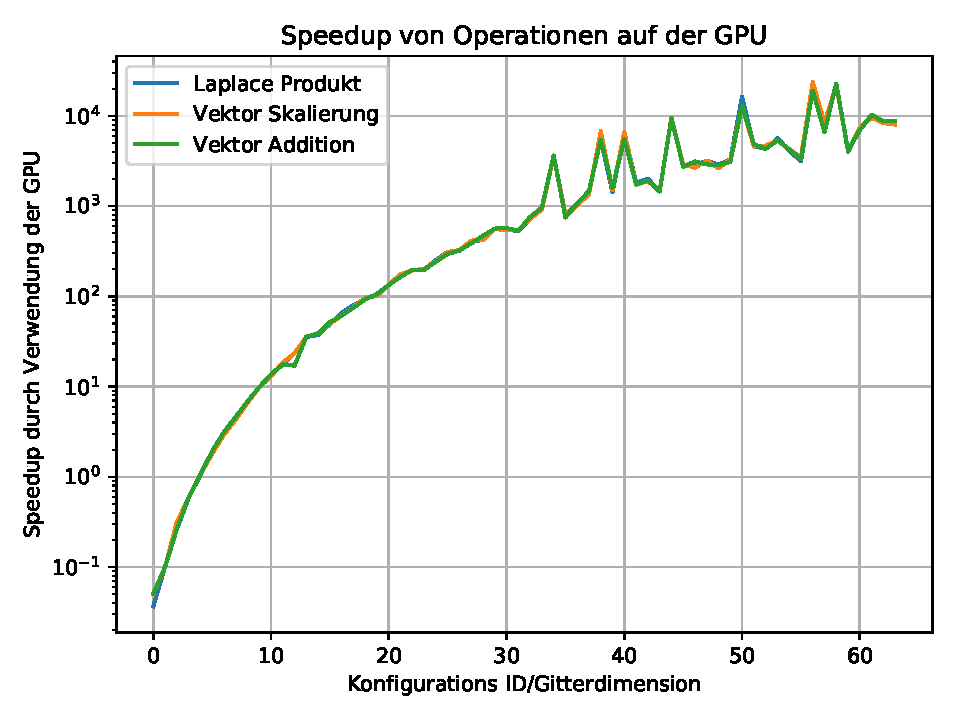
\includegraphics[width=.85\textwidth]{../aufg2/figures/speedup.pdf}
  \caption{
    Speedup der verschiedenen Funktionen in einem Semilogplot.
  }
  \label{fig:speedup}
\end{figure}

Während für kleine Gitter die Funktionen auf der CPU noch schneller ausgeführt werden, ist mit steigender Gitterdimension ein Speedup in der Größenordnung von $10^4$ erreichbar.
Während in Aufgabe 1 die execution configurations mit großen Blöcken und kleinen Threadanzahlen die schnellsten Laufzeiten erreichen, sieht man an
Abb. \ref{fig:speedup}, dass der Speedup für große Gitterdimensionen um eine Größenordnung fluktuiert.
Beispielsweise ist bei einer Gittergröße von \num{60} $\cdot$ \num{60}, einer Blockverteilung von \num{2}$\cdot$\num{2} und einer Threadverteilung
\num{31} $\cdot$ \num{31}  der Speedup bei ungefähr \num{20000}, während bei einer Blockverteillung von \num{5}$\cdot$\num{5} und einer Threadverteilung
\num{13} $\cdot$ \num{13}, für ein \num{63} $\cdot$ \num{63} Gitter, der Speedup nur bei etwa \num{7000} liegt.\\
In Aufgabe 1 jedoch waren gerade Kkonfigurationen mit vielen Blöcken und dafür wenigen Threads pro Block am schnellsten.
Im Gegensatz zu Aufgabe 1 waren die meisten Faktorisierungen jedoch recht symmetrisch, daher es war keine Block- oder Threaddimension deutlich größer als die jeweils andere.
\end{document}
